%%%%%%%%%%%%%%%%%%%%%%%%%%%%%%%%%%%%%%%%%
% Jacobs Landscape Poster
% LaTeX Template
% Version 1.1 (14/06/14)
%
% Created by:
% Computational Physics and Biophysics Group, Jacobs University
% https://teamwork.jacobs-university.de:8443/confluence/display/CoPandBiG/LaTeX+Poster
% 
% Further modified by:
% Nathaniel Johnston (nathaniel@njohnston.ca)
%
% This template has been downloaded from:
% http://www.LaTeXTemplates.com
%
% License:
% CC BY-NC-SA 3.0 (http://creativecommons.org/licenses/by-nc-sa/3.0/)
%
%%%%%%%%%%%%%%%%%%%%%%%%%%%%%%%%%%%%%%%%%

%----------------------------------------------------------------------------------------
%	PACKAGES AND OTHER DOCUMENT CONFIGURATIONS
%----------------------------------------------------------------------------------------

\documentclass[final]{beamer}
\usepackage{etoolbox}
\usepackage[scale=1.24]{beamerposter} % Use the beamerposter package for laying out the poster

\usetheme{confposter} % Use the confposter theme supplied with this template

\setbeamercolor{block title}{fg=BlueGreen,bg=white} % Colors of the block titles
\setbeamercolor{block body}{fg=black,bg=white} % Colors of the body of blocks
\setbeamercolor{block alerted title}{fg=white,bg=dblue!70} % Colors of the highlighted block titles
\setbeamercolor{block alerted body}{fg=black,bg=dblue!10} % Colors of the body of highlighted blocks
% Many more colors are available for use in beamerthemeconfposter.sty

%-----------------------------------------------------------
% Define the column widths and overall poster size
% To set effective sepwid, onecolwid and twocolwid values, first choose how many columns you want and how much separation you want between columns
% In this template, the separation width chosen is 0.024 of the paper width and a 4-column layout
% onecolwid should therefore be (1-(# of columns+1)*sepwid)/# of columns e.g. (1-(4+1)*0.024)/4 = 0.22
% Set twocolwid to be (2*onecolwid)+sepwid = 0.464
% Set threecolwid to be (3*onecolwid)+2*sepwid = 0.708

\makeatletter
\patchcmd{\beamer@@tmpl@headline}{wd=47in}{wd=71in}{}{}
\makeatother
\newlength{\sepwid}
\newlength{\onecolwid}
\newlength{\twocolwid}
\newlength{\threecolwid}
\setlength{\paperwidth}{72in} % A0 width: 46.8in
\setlength{\paperheight}{48in} % A0 height: 33.1in
\setlength{\sepwid}{0.024\paperwidth} % Separation width (white space) between columns
\setlength{\onecolwid}{0.22\paperwidth} % Width of one column
\setlength{\twocolwid}{0.464\paperwidth} % Width of two columns
\setlength{\threecolwid}{0.75\paperwidth} % Width of three columns
\setlength{\topmargin}{-1in} % Reduce the top margin size
%-----------------------------------------------------------

\usepackage{graphicx}  % Required for including images

\usepackage{booktabs} % Top and bottom rules for tables

%----------------------------------------------------------------------------------------
%	TITLE SECTION 
%----------------------------------------------------------------------------------------

\title{Cortical thickness and surface area as biomarkers to differentiate multiple sclerosis 
and neuromyelitis optica: a multivariate pattern classification study} % Poster title

\author{Arman Eshaghi, Viktor Wottschell, Maximiliano Calabrese, Daniel Alexander, Mohammad Ali Sahraian, Olga Ciccarelli} % Author(s)

\institute{MS Research Center, Neuroscience Institute, Tehran University of Medical Sciences, Terhan, Iran

Queen Square MS Centre, University College London (UCL) Institute of Neurology, London, United Kingdom

Centre for Medical Image Computing and Computer Science (CMIC), University College London, London, United Kingdom

Department of Neurological and Movement Sciences, University of Verona, Verona, Italy

\textbf{arman.eshaghi@me.com}} % Institution(s)



%----------------------------------------------------------------------------------------

\begin{document}

\addtobeamertemplate{block end}{}{\vspace*{2ex}} % White space under blocks
\addtobeamertemplate{block alerted end}{}{\vspace*{2ex}} % White space under highlighted (alert) blocks

\addtobeamertemplate{headline}{} 
{
\begin{tikzpicture}[remember picture,overlay] 
\node [shift={(10 cm,-13cm)}] at (current page.north west) {
\includegraphics[height=8cm]{Tums_logo.jpg}}; 
\end{tikzpicture} 
}
\addtobeamertemplate{headline}{} 
{
\begin{tikzpicture}[remember picture,overlay] 
\node [shift={(24 cm,-13cm)}] at (current page.north west) {
\includegraphics[height=8cm]{MSRC_logo.png}}; 
\end{tikzpicture} 
}

\addtobeamertemplate{headline}{} 
{
\begin{tikzpicture}[remember picture,overlay] 
\node [shift={(-10 cm,-13cm)}] at (current page.north east) {
\includegraphics[height=8cm]{UniVerona.jpg}}; 
\end{tikzpicture} 
}

\addtobeamertemplate{headline}{} 
{
\begin{tikzpicture}[remember picture,overlay] 
\node [shift={(-28 cm,-13cm)}] at (current page.north east) {
\includegraphics[height=8cm]{ucl-logo.jpg}}; 
\end{tikzpicture} 
}

\setlength{\belowcaptionskip}{2ex} % White space under figures
\setlength\belowdisplayshortskip{2ex} % White space under equations

\begin{frame}[t] % The whole poster is enclosed in one beamer frame

\begin{columns}[t] % The whole poster consists of three major columns, the second of which is split into two columns twice - the [t] option aligns each column's content to the top

\begin{column}{\sepwid}\end{column} % Empty spacer column

\begin{column}{\onecolwid} % The first column

%----------------------------------------------------------------------------------------
%	OBJECTIVES
%----------------------------------------------------------------------------------------

\begin{alertblock}{Objectives}


\begin{itemize}
\item To differentiate people with MS and NMO with measures from grey matter: cortical thickness and 
surface area, and volumes of deep grey matter nuclei
\item To investigate the pattern in which the above measures change in each disorder with multivariate statistical techniques

\end{itemize}

\end{alertblock}

%----------------------------------------------------------------------------------------
%	INTRODUCTION
%----------------------------------------------------------------------------------------

\begin{block}{Introduction}

Grey matter (GM) is affected in both multiple sclerosis (MS) and neuromyelitis optica (NMO) with different underlying mechanisms, and therefore it has been successfully used as a biomarker to discriminate NMO from MS (e.g. lesions detected with double-inversion recovery technique). 
However, it is still not clear whether the pattern in which GM changes occur in MS and NMO could be used to differentiate these  two disorders. We use cortical thickness and cortical surface area as two independent measures that could provide imoprtant information to differerntiate MS from NMO. Since it is important to have reproducible findings, we included two cohorts from two different countries. 



\end{block}

%------------------------------------------------

%----------------------------------------------------------------------------------------
%	MATERIALS
%----------------------------------------------------------------------------------------

\begin{block}{Setting and participants}

We included 97 subjects in two groups of people with MS and NMO, from the
cohorts in Tehran, Iran (25 patients with MS, and 30 patients with NMO) and Padua, 
Italy (24 patients with MS and 18 patients with NMO). Diagnosis was made for 
patients with MS based on 2005 revised McDonald criteria, and for patients with NMO 
according to 2006 Wingerchuk's criteria.

All patients underwent neurological examination to determine Expanded Disability 
Status Scale (EDSS). We performed MRI scan including high-resolution T1 (3D-
MPRAGE) and FLAIR with 1.5T in Padua and 3T scanners in Tehran.


\end{block}

\begin{block}{Image analysis(1)}

We calculated cortical thickness and area in 50 regions according to LONI probabilistic atlas (LPBA40). Cortical thickness was calculated with diffeomorphic based estimation of thickness in ANTs (DiReCT).

\begin{figure}
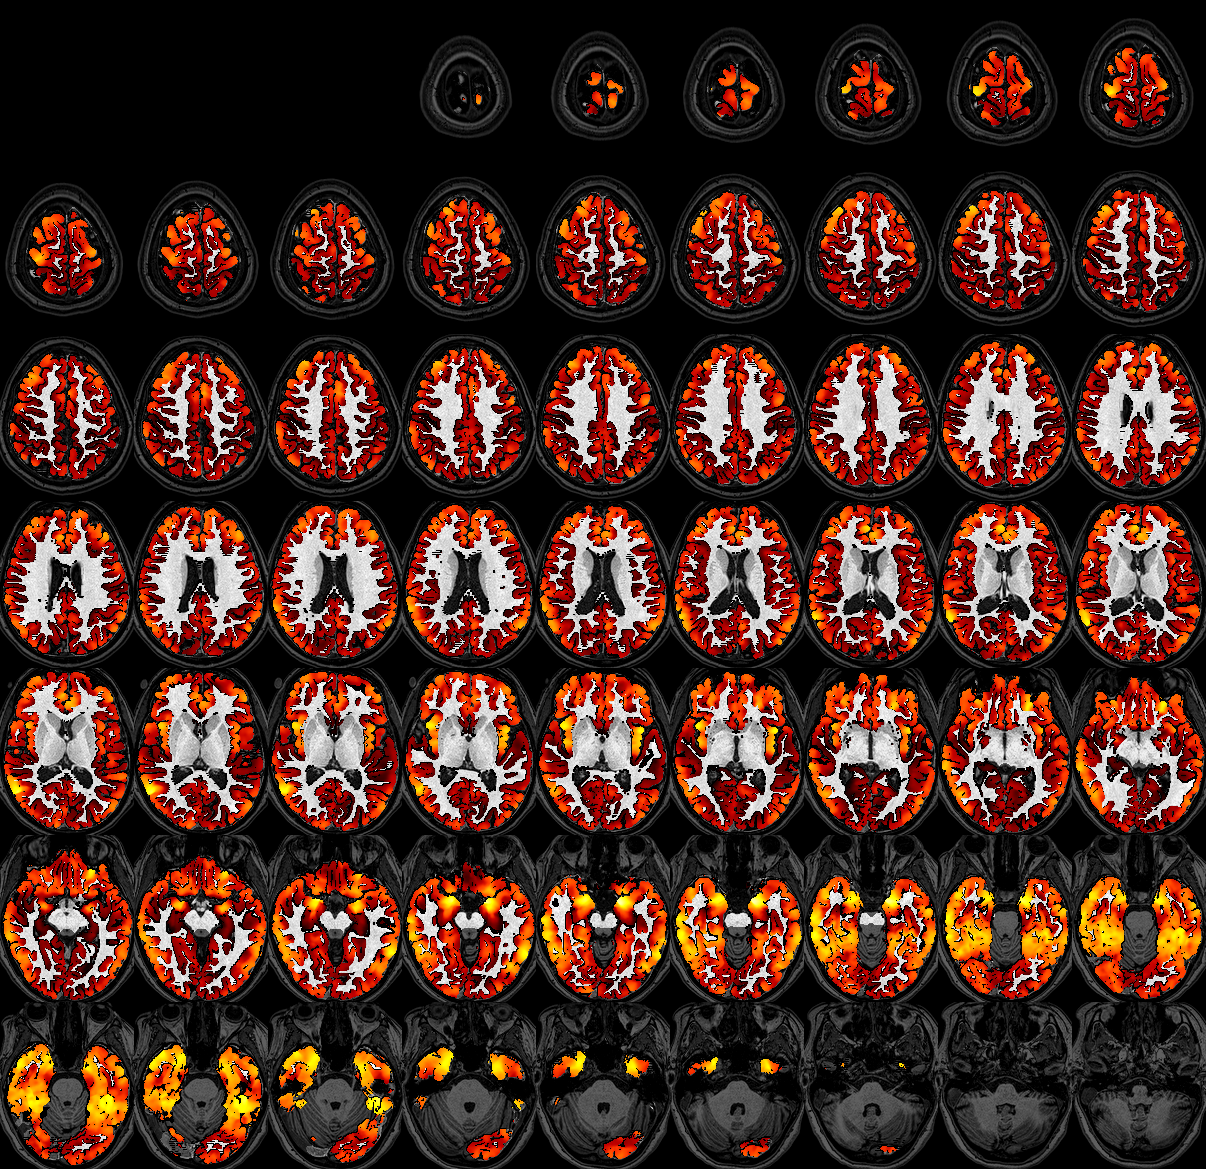
\includegraphics[width=0.9\linewidth]{NMO_THICKNESS_PAPER.png}
\caption{Cortical thickness map in a patient with NMO}
\end{figure}


\end{block}


%----------------------------------------------------------------------------------------

\end{column} % End of the first column

\begin{column}{\sepwid}\end{column} % Empty spacer column

\begin{column}{\twocolwid} % Begin a column which is two columns wide (column 2)

\begin{columns}[t,totalwidth=\twocolwid] % Split up the two columns wide column

\begin{column}{\onecolwid}\vspace{-.6in} % The first column within column 2 (column 2.1)


\begin{block}{Image analysis(2)}
To calculate \textbf{cortical volume} in each region of LPBA40 atlas we used Atropos to segment GM, and then calculated volumes. Cortical surface was then calculated in each region as follows:
  
\begin{equation}
Surface\,area = \frac{Volume}{Thickness}
\label{eqn:SurfaceEqn}
\end{equation}

We used FSL FIRST software to segment \textbf{deep grey matter nuclei}. FIRST uses a probabilistic Bayesian model on shape and 
intensity to automatically segment subcortical structures. Volumes of each structure were then calculated.
\end{block}

\begin{block}{Statistical analysis}
We used random forest technique as the method for classification. 
We randomly assigned each subject (from both cohorts) to training and test sets, 
so that each of sets will contain half of all patients. Next, we trained random forests 
on the training set and cross-validated on the left out half. This procedure was 
iterated for 5000 times. Mean and standard deviation for accuracy of 5000 trained 
and cross-validated models were calculated. Accuracy is defined as the sum of true 
positives (patients with MS classified as MS) and true negatives (patients with NMO 
classified as NMO) divided by all patients in the test set. To calculate the statistical 
significance of our classifier against null hypothesis (a random classifier) we used 
permutation testing P-value is defined 
as the number of times the random classifier has equal or more accuracy than the 
obtained accuracy from correct labels (MS or NMO) divided by 5000.

\end{block}

%----------------------------------------------------------------------------------------
%	RESULTS
%----------------------------------------------------------------------------------------


\begin{block}{Results}

Disease and demographic characteristics are shown in Figure 1.
Classifier with cortical volume gave 60\% classification accuracy, which was not different from a random classifier (P-value > 0.05).Classifier with cortical thickness gave 62\% (standard deviation = 0.11, p-value=0.03) accuracy. Feature importance as calculated inside random forest method is shown in Figure 2. Three most important regions to distinguish between two groups are: Left precuneus, left insular cortex, and the right fusiform gyrus.

The mean accuracy of the classifier with surface areas was 68\% (standard deviation = 0.13, P-value=0.03). Importance of each region in discrimination between two groups is shown in Figure 3. The three most important regions are: Left parahippocampal gyrus, right middle orbitofrontal gyrus, and right middle frontal gyrus.

The mean accuracy of the classifier when using subcortical volumes was 
72\% (standard deviation = 0.13, p-value = 0.03). Most important regions for differentiation were: the left thalamus, right pallidum, and right thalamus (Figure 4 and 5).

When using a combination of all measures from cortical thickness, surface and subcortical volumes, the mean accuracy reached 74\% (standard deviation = 0.10, P-value = 0.03) (Figure 6).




\begin{table}
\vspace{4ex}
\begin{tabular}{l l l}
\toprule
\textbf{Variables in classifier} & {Accuracy (p-value)}\\
\midrule
Cortical volume & 60\% (not significant) \\
Cortical thickness & 62\% (p=0.03) \\
Cortical surface & 72\% (p=0.03) \\
Subcortical volumes & 73\% (p=0.03) \\
Combination of all the above & 74\% (p=0.03) \\
\bottomrule
\end{tabular}
\caption{Classification results}
\end{table}

\end{block}

%----------------------------------------------------------------------------------------

\end{column} % End of column 2.1

\begin{column}{\onecolwid}\vspace{-.6in} % The second column within column 2 (column 2.2)

\begin{figure}
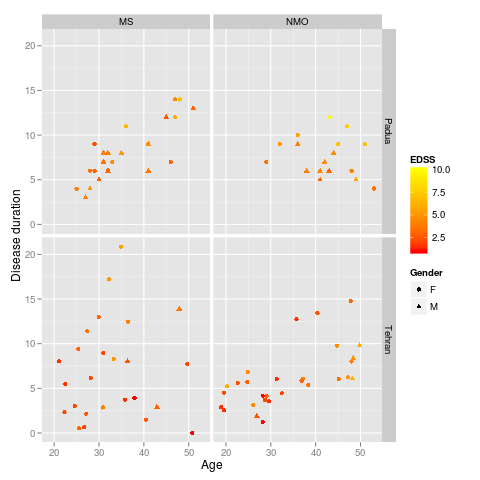
\includegraphics[width=0.6\linewidth]{descriptive_statistics_v2.png}
\caption{Disease and demographic characteristics in two cohorts from Iran and Italy}
\end{figure}

\begin{figure}
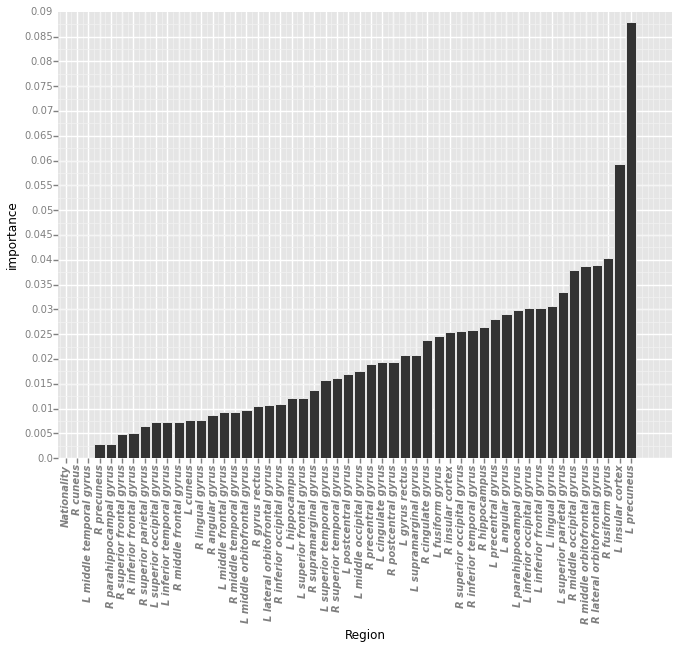
\includegraphics[width=0.7\linewidth]{v3_thickness_importance.png}
\caption{Importance of cortical thickness in each region to differentiate between NMO and MS}
\end{figure}

\begin{figure}
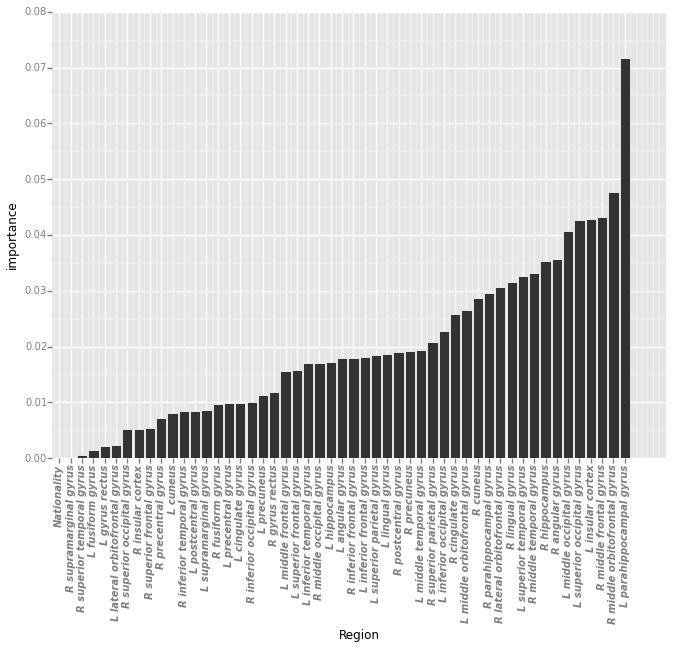
\includegraphics[width=0.7\linewidth]{v3_surface_importance.png}
\caption{Importance of cortical surface in each region to differentiate between NMO and MS}
\end{figure}



%----------------------------------------------------------------------------------------

\end{column} % End of column 2.2

\end{columns} % End of the split of column 2 - any content after this will now take up 2 columns width



\begin{columns}[t,totalwidth=\twocolwid] % Split up the two columns wide column again

\begin{column}{\onecolwid} % The first column within column 2 (column 2.1)


%----------------------------------------------------------------------------------------
%----------------------------------------------------------------------------------------

\end{column} % End of column 2.1

\begin{column}{\onecolwid} % The second column within column 2 (column 2.2)


%----------------------------------------------------------------------------------------

\end{column} % End of column 2.2

\end{columns} % End of the split of column 2

\end{column} % End of the second column

\begin{column}{\sepwid}\end{column} % Empty spacer column

\begin{column}{\onecolwid} % The third column


%----------------------------------------------------------------------------------------
%	ADDITIONAL INFORMATION
%----------------------------------------------------------------------------------------


\begin{figure}
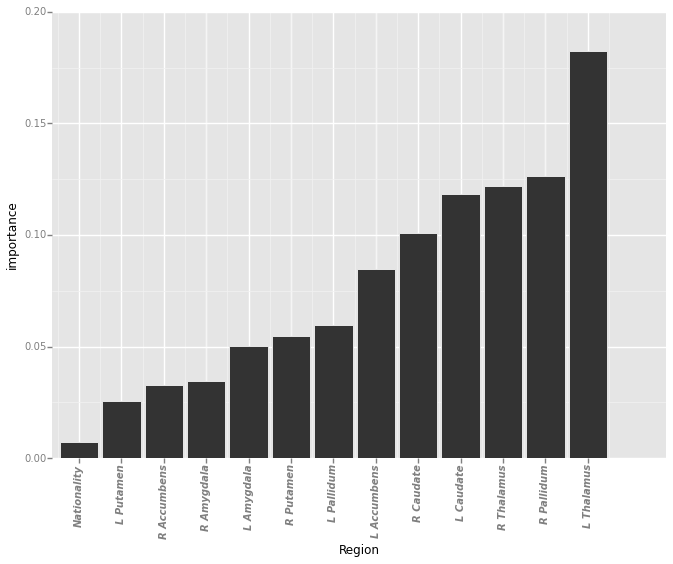
\includegraphics[width=0.7\linewidth]{v3_dgm_importance.png}
\caption{Importance of deep grey matter nuclei to differentiate between NMO and MS}
\end{figure}


\begin{figure}
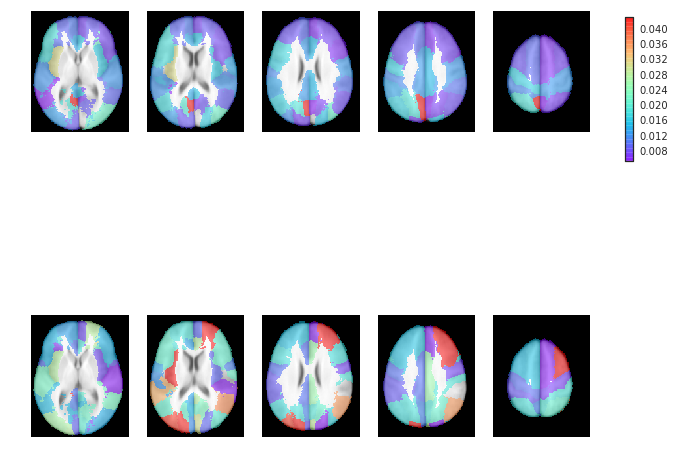
\includegraphics[width=0.7\linewidth]{v3_image_importance.png}
\caption{Imortance of cortical thickness (upper row) and surface area (lower row) to differentiate between MS and NMO in each region}
\end{figure}

\begin{block}{Summary of findings}

In this study we used multi-parameter classification approaches that combined cortical grey matter measures to investigate subtle differential changes in patients with MS and NMO. The classification was performed with random forests 
method, which had an accuracy of 62\%, 68\%, 73\% and 74\% in models using  cortical thickness, cortical surface, subcortical volumes, and combination of all those features, respectively. 
\end{block}

%----------------------------------------------------------------------------------------
%	CONCLUSION
%----------------------------------------------------------------------------------------

\begin{alertblock}{Conclusion}

\textbf{Cortical thickness}, \textbf{cortical surface} and \textbf{volumes of deep grey matter nuclei} provide up to 74 percent accuracy in discriminating MS from NMO. The results are reproducible across centers in different countries.

\end{alertblock} 

%----------------------------------------------------------------------------------------
%	REFERENCES
%----------------------------------------------------------------------------------------

\begin{block}{References}

\nocite{*} % Insert publications even if they are not cited in the poster
\small{\bibliographystyle{unsrt}
\bibliography{sample}\vspace{0.6in}}

\end{block}



%----------------------------------------------------------------------------------------

\end{column} % End of the third column

\end{columns} % End of all the columns in the poster

\end{frame} % End of the enclosing frame

\end{document}